\documentclass{beamer}

\usepackage{xspace}
\usepackage{tikz}
\usetikzlibrary{shapes,arrows}

\newcommand\javaPlex{\textsc{javaPlex}\xspace}
\newcommand\jPlex{\textsc{jPlex}\xspace}
\newcommand\Plex{\textsc{Plex}\xspace}

\begin{document}

\author{Andrew Tausz \and Mikael Vejdemo-Johansson}
\title{javaPlex -- persistent homology in Java}

\frame{\titlepage}

\begin{frame}
  \frametitle{Persistent homology}
  
  In a large variety of areas we encounter the following fundamental problem:

  \begin{block}{Problem}
    Estimate topological features of a shape based on a family of sample points (\emph{point clouds}).
  \end{block}
  \begin{block}{Applications}
    \begin{itemize}
    \item The space of natural $3\times3$ pixel patches is a Klein bottle.
    \item This Klein bottle yields new techniques for analyzing textures.
    \item Shape matching and shape databases.
    \item Filtering materials databases for high $CO_2$ adsorbitivity.
    \item Verifying sensor coverage for plane regions.
    \end{itemize}
  \end{block}
\end{frame}

\begin{frame}
  \frametitle{Persistent homology}
  
  Our favourite solution is due to Edelsbrunner, Letscher and Zomorodian.

  \begin{block}{Solution}
    \v Cech complexes, Vietoris-Rips complexes, $\alpha$-shapes and several other constructions capture by a filtered simplicial complex stemming from intersection relations of disks centered on the sample points

    \emph{Persistent homology} tracks the changes in topological features, and picks out such features that remain present over a long time.
  \end{block}
\end{frame}

\begin{frame}
  \frametitle{Persistent homology}
  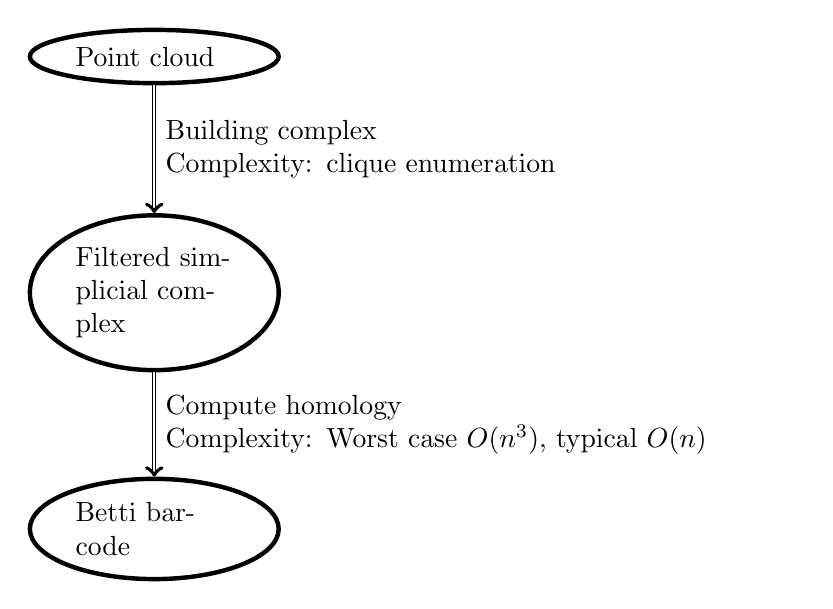
\begin{tikzpicture}[nodes={draw, ultra thick},node distance=3cm,text width=2cm]
    \node [ellipse] (pc) {Point cloud};
    \node [ellipse] (sc) [below of=pc] {Filtered simplicial complex};
    \node [ellipse] (bc) [below of=sc] {Betti barcode};
    \draw [->,double] (pc) -- node [right,draw=none,text width=8cm] {Building complex\\ Complexity: clique enumeration} (sc);
    \draw [->,double] (sc) -- node [right,draw=none,text width=8cm] {Compute homology\\ Complexity: Worst case $O(n^3)$, typical $O(n)$} (bc);
 \end{tikzpicture}
\end{frame}

\begin{frame}
  \frametitle{Vietoris-Rips complex}
  \begin{center}
    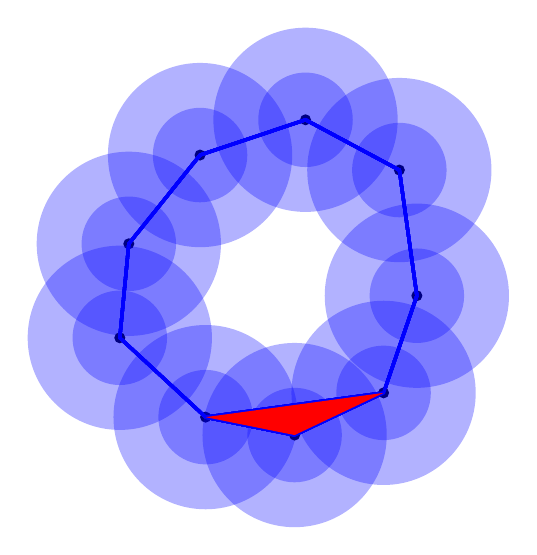
\begin{tikzpicture}[scale=2,very thick]
      \foreach \i/\x/\y in {%
        1/1.16585746601/0.0526160554712,%
        2/1.05457994334/0.850579088174,%
        3/0.458808003048/1.16969733378,%
        4/-0.210830688349/0.945845220034,%
        5/-0.663300962292/0.382325425778,%
        6/-0.720487145915/-0.214475039143,%
        7/-0.175593981068/-0.718417741544,%
        8/0.389575127029/-0.832215318256,%
        9/0.954490059554/-0.564264407025,%
        10/1.24416917416/0.298596099935,%
      }{ \node [coordinate] (n\i) at (\x,\y) {\i}; }

      \foreach \i in {1,2,3,4,5,6,7,8,9} { 
        \fill (n\i) circle (1pt);
        \fill<2-3> [blue,opacity=0.3] (n\i) circle (3mm);
        \draw<3> [blue] (n7) -- (n8);
        \fill<4-> [blue,opacity=0.3] (n\i) circle (5.85mm);
        \draw<5> [blue] (n1) -- (n2) -- (n3) -- (n4) -- (n5) -- (n6)
        -- (n7) -- (n8) -- (n9) -- (n1) (n7) -- (n9);
        \fill<5> [red] (n7) -- (n8) -- (n9) -- cycle;
      }
    \end{tikzpicture}
  \end{center}
\end{frame}


\begin{frame}
  \frametitle{History of \Plex}
  
  Early developments in the theory of persistent homology took place at Stanford, as did the development of software to compute with point clouds.

  \begin{enumerate}
  \item \Plex \only<2>{-- C++, Matlab through MEX, memory hog}
  \item \jPlex \only<2>{-- Java, Matlab natively, BeanShell, highly optimized}
  \end{enumerate}
\end{frame}

\begin{frame}
  \frametitle{Design properties for \javaPlex}
  
  \javaPlex grew out of dissatisfaction with both \Plex and \jPlex.

  \begin{block}{Disadvantages}
    \begin{columns}[t]
      \begin{column}{0.5\textwidth}
        \Plex
        \begin{itemize}
        \item Dependent on exact Matlab version and \textsc{mex} dialect
        \item Design carrying \emph{very} many pointers: high memory consumption
        \end{itemize}
      \end{column}
      \begin{column}{0.5\textwidth}
        \jPlex
        \begin{itemize}
        \item Too highly optimized: no real capacity to extend or modify
        \item Not actually competitive enough to motivate this
        \end{itemize}
      \end{column}
    \end{columns}
  \end{block}
\end{frame}

\begin{frame}
  \frametitle{Usage examples}
  
  This is joint work with David Eklund, Jonathan Hauenstein, Martina Scolamiero, and Chris Peterson.

  \begin{block}{Application}
    Consider as a linkage the configurations of cyclo-octane ($C_8H_{16}$). 
    The carbon bonds in this have fixed length, and an angle of $\arccos(-1/3)\simeq 109.47º$.
    By fixing one carbon atom at the origin, and it's closest neighbours at $(1,0,0)$ and $(-\frac13,\frac23\sqrt{2},0)$, we may study the distribution of the remaining atoms.
    The variety of possible configurations is a surface in $\mathbb R^{15}$.
  \end{block}
  This variety was first described by \textit{Martin, Thompson, Coutsias, and Watson} in \textsc{Topology of cyclo-octane energy landscape}. J. Chem. Phys. 132, 234115 (2010).
\end{frame}

\begin{frame}
  \frametitle{Cyclo-octane}
  We sample, using \textsc{Bertini}, points on the real singular locus of the cyclo-octane variety.

  Using \textsc{Matlab} and \javaPlex, we create a witness complex on 100 out of 1\,606 sampled points:
\end{frame}

\begin{frame}[fragile]
  \frametitle{Cyclo-octane}
{\fontsize{9pt}{14pt}
\begin{verbatim}
>> load Distances.out;
>> m_space = metric.impl.ExplicitMetricSpace(Distances);
>> diam = metric.utility.MetricUtility.estimateDiameter(m_space);
>> r_max = diam/2
ans = 3.1017
>> landmarks = api.Plex4.createMaxMinSelector(m_space,100);
>> stream = api.Plex4.createWitnessStream(landmarks,3,r_max/2);
>> stream.getSize()
ans = 11418
>> persistence = api.Plex4.getDefaultSimplicialAlgorithm(3);
>> fii = persistence.computeIntervals(stream);
>> fvi = stream.transform(fii);
>> api.Plex4.createBarcodePlot(fvi,'witness',r_max/2);
\end{verbatim}
}
\end{frame}

\begin{frame}
  \frametitle{Cyclo-octane}
  From the Matlab code above, we acquire the Betti barcodes:

  \noindent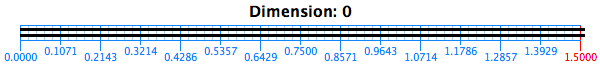
\includegraphics[width=\textwidth]{witness_0} \\
  \noindent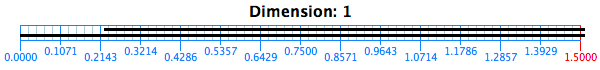
\includegraphics[width=\textwidth]{witness_1} 

  Which is strongly consistent with the structure of the singular set from \textit{Martin, Thompson, Coutsias, and Watson} as a pair of disjoint circles.

  The entire computation runs in 6 seconds. (mean running time for 10 runs, std.dev. 0.8s)
\end{frame}

\begin{frame}
  \frametitle{Cyclo-octane}

  \begin{columns}
    \begin{column}{0.6\textwidth}
      \begin{itemize}
      \item Computation with coefficients in $\mathbb F_2$ and $\mathbb F_3$ to look for torsion.
      \item Witness complex with 500 landmarks.
      \item Total complex 26M simplices.
      \item Computation time: 3 days.
      \item Severe memory issues.
      \item Surprising lack of difference between $\mathbb F_2$ and $\mathbb F_3$: torsion killed by particular intersection of sphere and Klein bottle.
      \end{itemize}
    \end{column}
    \begin{column}{0.3\textwidth}
      \noindent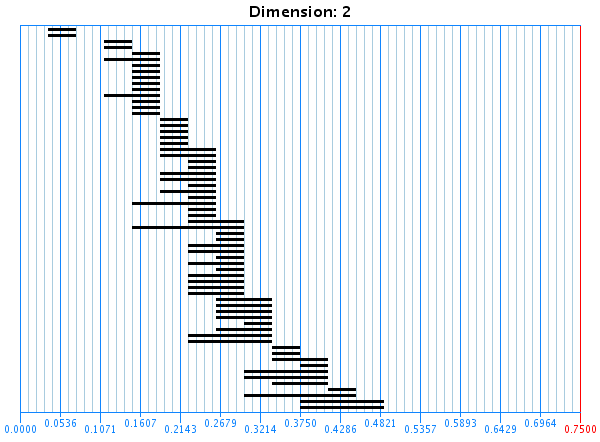
\includegraphics[width=\textwidth]{cyclo8ane2_2} \\
      \noindent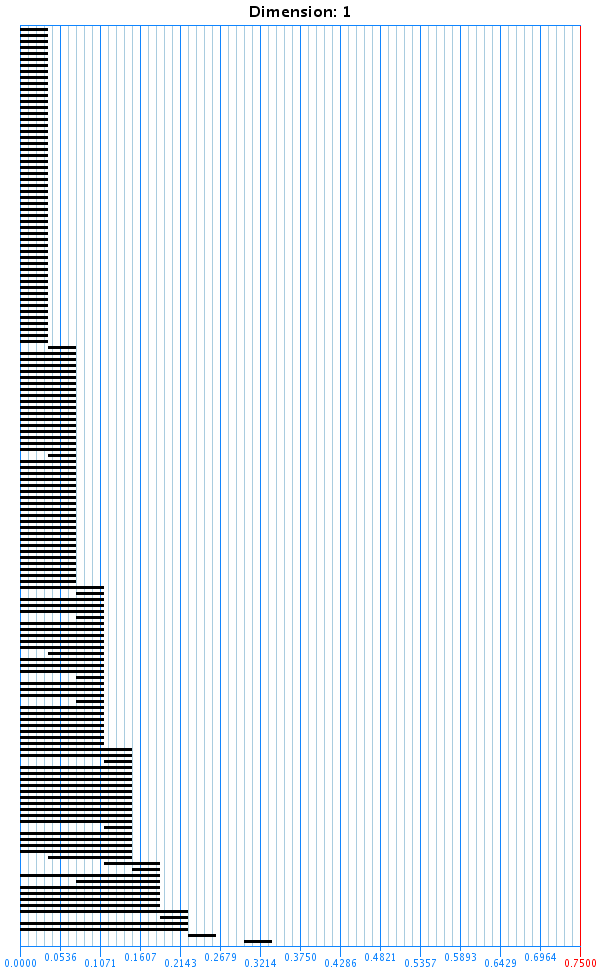
\includegraphics[width=\textwidth]{cyclo8ane2_1} \\
      \noindent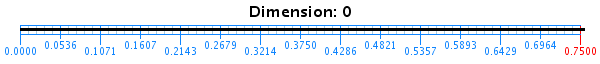
\includegraphics[width=\textwidth]{cyclo8ane2_0} \\
    \end{column}
  \end{columns}

\end{frame}

\begin{frame}
  \frametitle{Access to the package}
  
  \begin{block}{Software package}
    Published on \url{http://code.google.com/p/javaplex}
  \end{block}

  \begin{block}{JavaDoc documentation}
    Linked from software homepage.
  \end{block}

  \begin{block}{Usage tutorial}
    Linked from software homepage. Thanks to Henry Adams for adapting the jPlex tutorial to javaPlex.
  \end{block}

  Questions or comments?
\end{frame}

\end{document}

%%% Local Variables: 
%%% mode: latex
%%% TeX-master: t
%%% End: 
